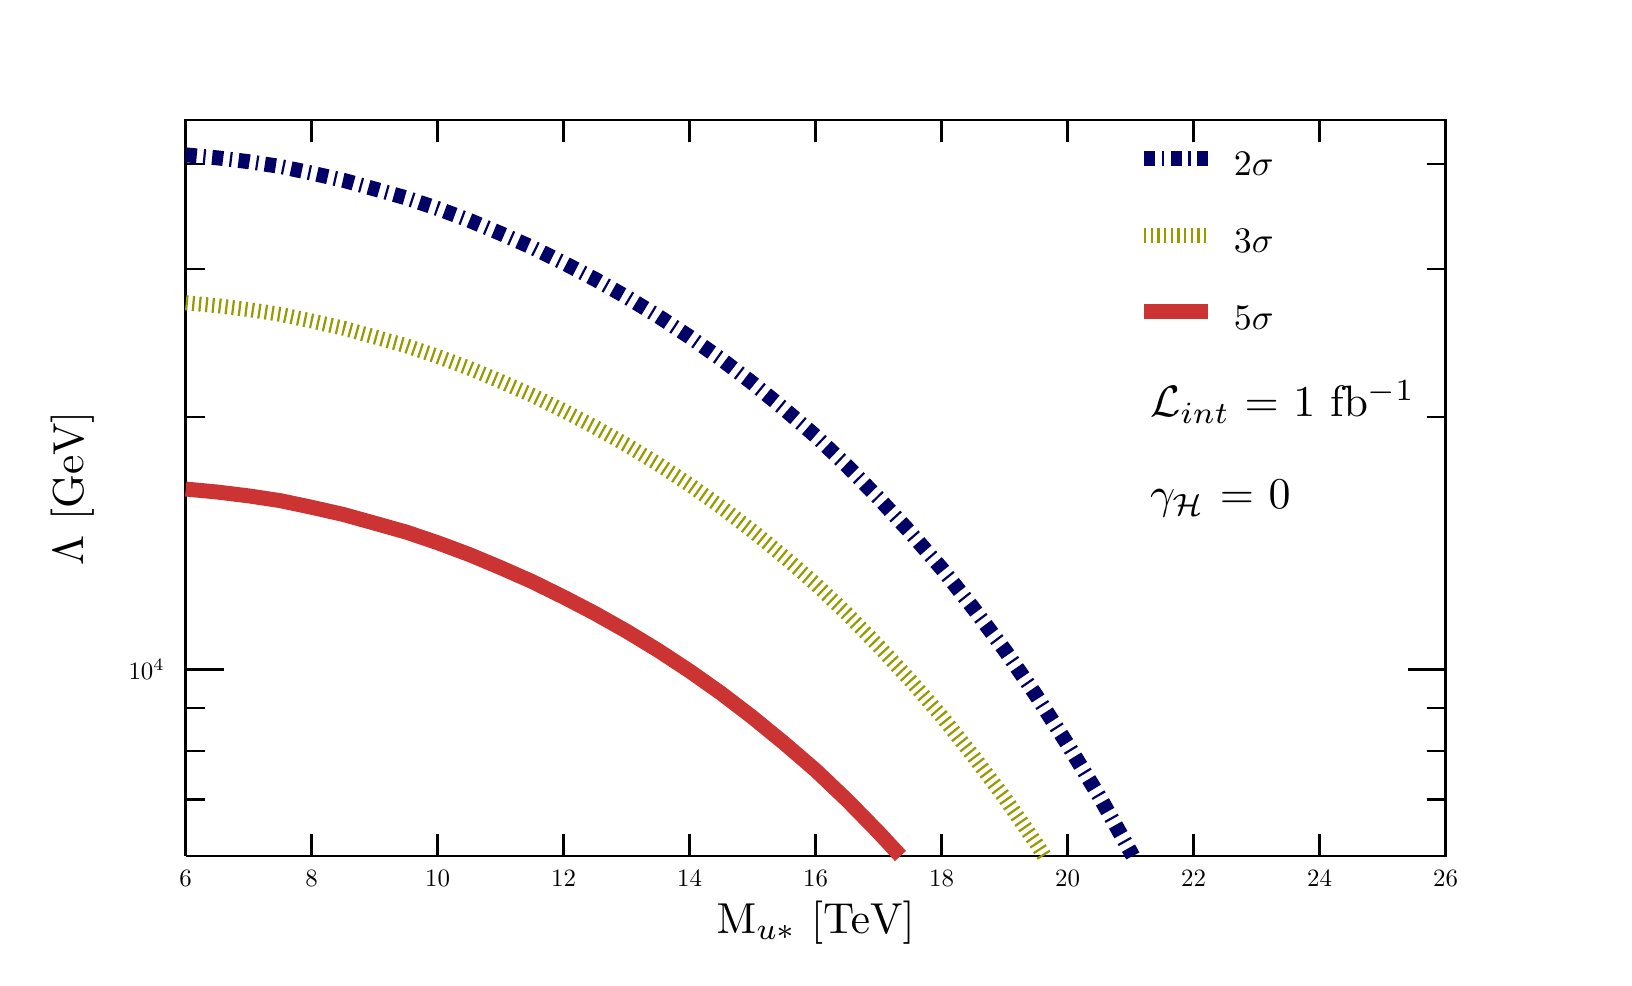
\begin{tikzpicture}
\pgfdeclareplotmark{cross} {
\pgfpathmoveto{\pgfpoint{-0.3\pgfplotmarksize}{\pgfplotmarksize}}
\pgfpathlineto{\pgfpoint{+0.3\pgfplotmarksize}{\pgfplotmarksize}}
\pgfpathlineto{\pgfpoint{+0.3\pgfplotmarksize}{0.3\pgfplotmarksize}}
\pgfpathlineto{\pgfpoint{+1\pgfplotmarksize}{0.3\pgfplotmarksize}}
\pgfpathlineto{\pgfpoint{+1\pgfplotmarksize}{-0.3\pgfplotmarksize}}
\pgfpathlineto{\pgfpoint{+0.3\pgfplotmarksize}{-0.3\pgfplotmarksize}}
\pgfpathlineto{\pgfpoint{+0.3\pgfplotmarksize}{-1.\pgfplotmarksize}}
\pgfpathlineto{\pgfpoint{-0.3\pgfplotmarksize}{-1.\pgfplotmarksize}}
\pgfpathlineto{\pgfpoint{-0.3\pgfplotmarksize}{-0.3\pgfplotmarksize}}
\pgfpathlineto{\pgfpoint{-1.\pgfplotmarksize}{-0.3\pgfplotmarksize}}
\pgfpathlineto{\pgfpoint{-1.\pgfplotmarksize}{0.3\pgfplotmarksize}}
\pgfpathlineto{\pgfpoint{-0.3\pgfplotmarksize}{0.3\pgfplotmarksize}}
\pgfpathclose
\pgfusepathqstroke
}
\pgfdeclareplotmark{cross*} {
\pgfpathmoveto{\pgfpoint{-0.3\pgfplotmarksize}{\pgfplotmarksize}}
\pgfpathlineto{\pgfpoint{+0.3\pgfplotmarksize}{\pgfplotmarksize}}
\pgfpathlineto{\pgfpoint{+0.3\pgfplotmarksize}{0.3\pgfplotmarksize}}
\pgfpathlineto{\pgfpoint{+1\pgfplotmarksize}{0.3\pgfplotmarksize}}
\pgfpathlineto{\pgfpoint{+1\pgfplotmarksize}{-0.3\pgfplotmarksize}}
\pgfpathlineto{\pgfpoint{+0.3\pgfplotmarksize}{-0.3\pgfplotmarksize}}
\pgfpathlineto{\pgfpoint{+0.3\pgfplotmarksize}{-1.\pgfplotmarksize}}
\pgfpathlineto{\pgfpoint{-0.3\pgfplotmarksize}{-1.\pgfplotmarksize}}
\pgfpathlineto{\pgfpoint{-0.3\pgfplotmarksize}{-0.3\pgfplotmarksize}}
\pgfpathlineto{\pgfpoint{-1.\pgfplotmarksize}{-0.3\pgfplotmarksize}}
\pgfpathlineto{\pgfpoint{-1.\pgfplotmarksize}{0.3\pgfplotmarksize}}
\pgfpathlineto{\pgfpoint{-0.3\pgfplotmarksize}{0.3\pgfplotmarksize}}
\pgfpathclose
\pgfusepathqfillstroke
}
\pgfdeclareplotmark{newstar} {
\pgfpathmoveto{\pgfqpoint{0pt}{\pgfplotmarksize}}
\pgfpathlineto{\pgfqpointpolar{44}{0.5\pgfplotmarksize}}
\pgfpathlineto{\pgfqpointpolar{18}{\pgfplotmarksize}}
\pgfpathlineto{\pgfqpointpolar{-20}{0.5\pgfplotmarksize}}
\pgfpathlineto{\pgfqpointpolar{-54}{\pgfplotmarksize}}
\pgfpathlineto{\pgfqpointpolar{-90}{0.5\pgfplotmarksize}}
\pgfpathlineto{\pgfqpointpolar{234}{\pgfplotmarksize}}
\pgfpathlineto{\pgfqpointpolar{198}{0.5\pgfplotmarksize}}
\pgfpathlineto{\pgfqpointpolar{162}{\pgfplotmarksize}}
\pgfpathlineto{\pgfqpointpolar{134}{0.5\pgfplotmarksize}}
\pgfpathclose
\pgfusepathqstroke
}
\pgfdeclareplotmark{newstar*} {
\pgfpathmoveto{\pgfqpoint{0pt}{\pgfplotmarksize}}
\pgfpathlineto{\pgfqpointpolar{44}{0.5\pgfplotmarksize}}
\pgfpathlineto{\pgfqpointpolar{18}{\pgfplotmarksize}}
\pgfpathlineto{\pgfqpointpolar{-20}{0.5\pgfplotmarksize}}
\pgfpathlineto{\pgfqpointpolar{-54}{\pgfplotmarksize}}
\pgfpathlineto{\pgfqpointpolar{-90}{0.5\pgfplotmarksize}}
\pgfpathlineto{\pgfqpointpolar{234}{\pgfplotmarksize}}
\pgfpathlineto{\pgfqpointpolar{198}{0.5\pgfplotmarksize}}
\pgfpathlineto{\pgfqpointpolar{162}{\pgfplotmarksize}}
\pgfpathlineto{\pgfqpointpolar{134}{0.5\pgfplotmarksize}}
\pgfpathclose
\pgfusepathqfillstroke
}
\definecolor{c}{rgb}{1,1,1};
\draw [color=c, fill=c] (0,0) rectangle (20,11.6806);
\draw [color=c, fill=c] (2,1.16806) rectangle (18,10.5125);
\definecolor{c}{rgb}{0,0,0};
\draw [c,line width=0.9] (2,1.16806) -- (2,10.5125) -- (18,10.5125) -- (18,1.16806) -- (2,1.16806);
\definecolor{c}{rgb}{1,1,1};
\draw [color=c, fill=c] (2,1.16806) rectangle (18,10.5125);
\definecolor{c}{rgb}{0,0,0};
\draw [c,line width=0.9] (2,1.16806) -- (2,10.5125) -- (18,10.5125) -- (18,1.16806) -- (2,1.16806);
\draw [c,line width=0.9] (2,1.16806) -- (18,1.16806);
\draw (10,0.327056) node[scale=1.56475, color=c, rotate=0]{M$_{u*}$ [TeV]};
\draw [c,line width=0.9] (2,1.44839) -- (2,1.16806);
\draw [c,line width=0.9] (3.6,1.44839) -- (3.6,1.16806);
\draw [c,line width=0.9] (5.2,1.44839) -- (5.2,1.16806);
\draw [c,line width=0.9] (6.8,1.44839) -- (6.8,1.16806);
\draw [c,line width=0.9] (8.4,1.44839) -- (8.4,1.16806);
\draw [c,line width=0.9] (10,1.44839) -- (10,1.16806);
\draw [c,line width=0.9] (11.6,1.44839) -- (11.6,1.16806);
\draw [c,line width=0.9] (13.2,1.44839) -- (13.2,1.16806);
\draw [c,line width=0.9] (14.8,1.44839) -- (14.8,1.16806);
\draw [c,line width=0.9] (16.4,1.44839) -- (16.4,1.16806);
\draw [c,line width=0.9] (18,1.44839) -- (18,1.16806);
\draw [anchor=base] (2,0.782598) node[scale=0.900036, color=c, rotate=0]{6};
\draw [anchor=base] (3.6,0.782598) node[scale=0.900036, color=c, rotate=0]{8};
\draw [anchor=base] (5.2,0.782598) node[scale=0.900036, color=c, rotate=0]{10};
\draw [anchor=base] (6.8,0.782598) node[scale=0.900036, color=c, rotate=0]{12};
\draw [anchor=base] (8.4,0.782598) node[scale=0.900036, color=c, rotate=0]{14};
\draw [anchor=base] (10,0.782598) node[scale=0.900036, color=c, rotate=0]{16};
\draw [anchor=base] (11.6,0.782598) node[scale=0.900036, color=c, rotate=0]{18};
\draw [anchor=base] (13.2,0.782598) node[scale=0.900036, color=c, rotate=0]{20};
\draw [anchor=base] (14.8,0.782598) node[scale=0.900036, color=c, rotate=0]{22};
\draw [anchor=base] (16.4,0.782598) node[scale=0.900036, color=c, rotate=0]{24};
\draw [anchor=base] (18,0.782598) node[scale=0.900036, color=c, rotate=0]{26};
\draw [c,line width=0.9] (2,10.5125) -- (18,10.5125);
\draw [c,line width=0.9] (2,10.2322) -- (2,10.5125);
\draw [c,line width=0.9] (3.6,10.2322) -- (3.6,10.5125);
\draw [c,line width=0.9] (5.2,10.2322) -- (5.2,10.5125);
\draw [c,line width=0.9] (6.8,10.2322) -- (6.8,10.5125);
\draw [c,line width=0.9] (8.4,10.2322) -- (8.4,10.5125);
\draw [c,line width=0.9] (10,10.2322) -- (10,10.5125);
\draw [c,line width=0.9] (11.6,10.2322) -- (11.6,10.5125);
\draw [c,line width=0.9] (13.2,10.2322) -- (13.2,10.5125);
\draw [c,line width=0.9] (14.8,10.2322) -- (14.8,10.5125);
\draw [c,line width=0.9] (16.4,10.2322) -- (16.4,10.5125);
\draw [c,line width=0.9] (18,10.2322) -- (18,10.5125);
\draw [c,line width=0.9] (2,1.16806) -- (2,10.5125);
\draw (0.56,5.84029) node[scale=1.56475, color=c, rotate=90]{$\Lambda$ [GeV]};
\draw [c,line width=0.9] (2.24,1.16882) -- (2,1.16882);
\draw [c,line width=0.9] (2.24,1.88283) -- (2,1.88283);
\draw [c,line width=0.9] (2.24,2.50134) -- (2,2.50134);
\draw [c,line width=0.9] (2.24,3.0469) -- (2,3.0469);
\draw [c,line width=0.9] (2.48,3.53492) -- (2,3.53492);
\draw [anchor= east] (1.844,3.53492) node[scale=0.900036, color=c, rotate=0]{$10^{4}$};
\draw [c,line width=0.9] (2.24,6.74553) -- (2,6.74553);
\draw [c,line width=0.9] (2.24,8.62361) -- (2,8.62361);
\draw [c,line width=0.9] (2.24,9.95613) -- (2,9.95613);
\draw [c,line width=0.9] (18,1.16806) -- (18,10.5125);
\draw [c,line width=0.9] (17.76,1.16882) -- (18,1.16882);
\draw [c,line width=0.9] (17.76,1.88283) -- (18,1.88283);
\draw [c,line width=0.9] (17.76,2.50134) -- (18,2.50134);
\draw [c,line width=0.9] (17.76,3.0469) -- (18,3.0469);
\draw [c,line width=0.9] (17.52,3.53492) -- (18,3.53492);
\draw [c,line width=0.9] (17.76,6.74553) -- (18,6.74553);
\draw [c,line width=0.9] (17.76,8.62361) -- (18,8.62361);
\draw [c,line width=0.9] (17.76,9.95613) -- (18,9.95613);
\definecolor{c}{rgb}{0,0,0.4};
\draw [c,dash pattern=on 4.00pt off 2.40pt on 0.80pt off 2.40pt ,line width=5.4] (2,10.0722) -- (2.4,10.0345) -- (2.8,9.98551) -- (3.2,9.92521) -- (3.6,9.84073) -- (4,9.75003) -- (4.4,9.63868) -- (4.8,9.52598) -- (5.2,9.3906) -- (5.6,9.24124) --
 (6,9.07397) -- (6.4,8.89692) -- (6.8,8.70036) -- (7.2,8.49182) -- (7.6,8.26627) -- (8,8.02328) -- (8.4,7.76038) -- (8.8,7.47814) -- (9.2,7.17254) -- (9.6,6.84533) -- (10,6.50077) -- (10.4,6.12056) -- (10.8,5.71181) -- (11.2,5.27978) --
 (11.6,4.81992) -- (12,4.318) -- (12.4,3.78543) -- (12.8,3.2084) -- (13.2,2.58463) -- (13.6,1.92969) -- (14,1.22054) -- (14.0276,1.16806);
\definecolor{c}{rgb}{0.6,0.6,0};
\draw [c,dash pattern=on 0.80pt off 1.60pt ,line width=5.4] (2,8.19415) -- (2.4,8.15642) -- (2.8,8.10742) -- (3.2,8.04712) -- (3.6,7.96265) -- (4,7.87197) -- (4.4,7.76061) -- (4.8,7.6479) -- (5.2,7.51252) -- (5.6,7.36316) -- (6,7.1959) --
 (6.4,7.01884) -- (6.8,6.82227) -- (7.2,6.61373) -- (7.6,6.3882) -- (8,6.1452) -- (8.4,5.8823) -- (8.8,5.60008) -- (9.2,5.29448) -- (9.6,4.96724) -- (10,4.6227) -- (10.4,4.24248) -- (10.8,3.83375) -- (11.2,3.40169) -- (11.6,2.94182) -- (12,2.43992)
 -- (12.4,1.90735) -- (12.8,1.33032) -- (12.9041,1.16806);
\definecolor{c}{rgb}{0.8,0.2,0.2};
\draw [c,line width=5.4] (2,5.82805) -- (2.4,5.79032) -- (2.8,5.74133) -- (3.2,5.68102) -- (3.6,5.59655) -- (4,5.50586) -- (4.4,5.39451) -- (4.8,5.28179) -- (5.2,5.14641) -- (5.6,4.99706) -- (6,4.8298) -- (6.4,4.65271) -- (6.8,4.45618) --
 (7.2,4.24761) -- (7.6,4.02211) -- (8,3.77911) -- (8.4,3.51619) -- (8.8,3.23397) -- (9.2,2.92836) -- (9.6,2.60115) -- (10,2.2566) -- (10.4,1.87638) -- (10.8,1.46763) -- (11.0774,1.16806);
\definecolor{c}{rgb}{0,0,0};
\draw (10,11.301) node[scale=1.2177, color=c, rotate=0]{ };
\draw [anchor=base west] (15.15,9.80681) node[scale=1.29711, color=c, rotate=0]{$2\sigma$};
\definecolor{c}{rgb}{0,0,0.4};
\draw [c,dash pattern=on 4.00pt off 2.40pt on 0.80pt off 2.40pt ,line width=5.4] (14.1725,10.0258) -- (14.9775,10.0258);
\definecolor{c}{rgb}{0,0,0};
\draw [anchor=base west] (15.15,8.83343) node[scale=1.29711, color=c, rotate=0]{$3\sigma$};
\definecolor{c}{rgb}{0.6,0.6,0};
\draw [c,dash pattern=on 0.80pt off 1.60pt ,line width=5.4] (14.1725,9.05244) -- (14.9775,9.05244);
\definecolor{c}{rgb}{0,0,0};
\draw [anchor=base west] (15.15,7.86005) node[scale=1.29711, color=c, rotate=0]{$5\sigma$};
\definecolor{c}{rgb}{0.8,0.2,0.2};
\draw [c,line width=5.4] (14.1725,8.07906) -- (14.9775,8.07906);
\definecolor{c}{rgb}{0,0,0};
\draw [anchor=base west] (14.05,6.74553) node[scale=1.5883, color=c, rotate=0]{$\mathcal{L}_{int}$ = 1 fb$^{-1}$};
\draw [anchor=base west] (14.05,5.57747) node[scale=1.5883, color=c, rotate=0]{$\gamma_{\mathcal{H}}$ = 0};
\end{tikzpicture}
